\begin{example}[Définition 10 : $a > b$ : $a = 7$, $b = 3$]
    ~
    \begin{itemize}
        \item Limites pour toute séquence de $\mathcal{PF}_{7,3}$
            une fois triée : $[1,\ 1 \frac{3}{7},\ 1 \frac{6}{7},\ 
            2 \frac{2}{7},\ 2 \frac{5}{7},\ 3 \frac{1}{7},\ 
            3 \frac{4}{7}]$
        \item $f_1 = (2, 1, 1, 3, 2, 3, 1) \in
            \mathcal{PF}_{7,3}$
        \item $f_2 = (2, 1, 2, 3, 2, 3, 1) \notin
            \mathcal{PF}_{7,3}$, bien que $f_2 \in
            \mathcal{PF}_7$
    \end{itemize}
\end{example}

\begin{example}[Définition 10 : $a < b$ : $a = 5$, $b = 7$]
    ~
    \begin{itemize}
        \item Limites pour toute séquence de $\mathcal{PF}_{5,7}$
            une fois triée : $[1,\ 2 \frac{2}{5},\ 3 \frac{4}{5},\ 
            5 \frac{1}{5},\ 6 \frac{3}{5}]$
        \item $f_3 = (6, 3, 5, 1, 2) \in
            \mathcal{PF}_{5,7}$, bien que $f_3 \notin
            \mathcal{PF}_5$
        \item $f_4 = (6, 3, 5, 1, 3) \notin
            \mathcal{PF}_{5,7}$\\
    \end{itemize}
\end{example}

\begin{example}[Théorème 6 : $a = 3, b = 5$]
    ~\\
    \begin{itemize*}\\
        \item $pf_{a,b} = 25$
        \item Limites : $[1,\ 2 \frac{2}{3},\ 
            4 \frac{1}{3}]$\\\\
        \subitem $(1, 1, 1)$
        \subitem $(1, 1, 2)$
        \subitem $(1, 1, 3)$
        \subitem $(1, 1, 4)$
        \subitem $(1, 2, 1)$
        \subitem $(1, 2, 2)$
        \subitem $(1, 2, 3)$
        \subitem $(1, 2, 4)$
        \subitem $(1, 3, 1)$
        \subitem $(1, 3, 2)$
        \subitem $(1, 4, 1)$
        \subitem $(1, 4, 2)$
        \subitem $(2, 1, 1)$
        \subitem $(2, 1, 2)$
        \subitem $(2, 1, 3)$
        \subitem $(2, 1, 4)$
        \subitem $(2, 2, 1)$
        \subitem $(2, 3, 1)$
        \subitem $(2, 4, 1)$
        \subitem $(3, 1, 1)$
        \subitem $(3, 1, 2)$
        \subitem $(3, 2, 1)$
        \subitem $(4, 1, 1)$
        \subitem $(4, 1, 2)$
        \subitem $(4, 2, 1)$\\
    \end{itemize*}
\end{example}

\begin{example}[Définition 11 : $a < b : a = 3, b = 5$]
    ~
    \begin{itemize}
        \item $w_1 = 10100010 \text{ n'est \emph{pas} un 3, 5 - mot de
        Dyck, car } |101000|_1 = 2 < \frac{3}{5}|101000|_0 = 2 \frac{2}{5}.$
        \item $w_2 = 10100100 \text{ \emph{est} un 3, 5 - mot de Dyck : }$
    \end{itemize}
    \begin{center}
    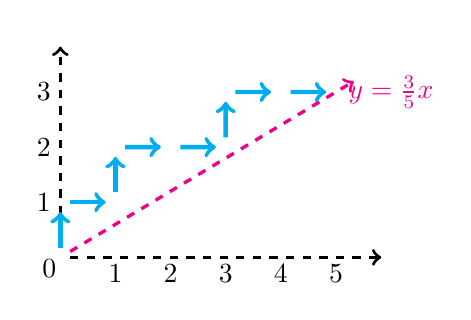
\begin{tikzpicture}[scale=0.7]
        \node (a) at (0, 0) {};
        \node (b) at (0, 4) {};
        \node (c) at (6, 0) {};
        \node (d) at (5.5, 3.3) {};
        \node (e) at (6, 3) [color = magenta]
            {$y = \frac{3}{5}x$}; 
        \draw [dashed, very thick, ->] (a) to (b);
        \draw [dashed, very thick, ->] (a) to (c);
        \draw [dashed, very thick, ->]
            [color = magenta] (a) to (d);

        \node (1)  at (0,0)   {};
        \node (2)  at (0,1)   {};
        \node (3)  at (1,1)   {};
        \node (4)  at (1,2)   {};
        \node (5)  at (2,2)   {};
        \node (6)  at (3,2)   {};
        \node (7)  at (3,3)   {};
        \node (8)  at (4,3)   {};
        \node (9)  at (5,3)   {};
        \draw [->, ultra thick, color = cyan]
            (1)  to (2);
        \draw [->, ultra thick, color = cyan] 
            (2)  to (3);
        \draw [->, ultra thick, color = cyan]
            (3)  to (4);
        \draw [->, ultra thick, color = cyan]
            (4)  to (5);
        \draw [->, ultra thick, color = cyan]
            (5)  to (6);
        \draw [->, ultra thick, color = cyan]
            (6)  to (7);
        \draw [->, ultra thick, color = cyan]
            (7)  to (8);
        \draw [->, ultra thick, color = cyan]
            (8)  to (9);

        \node at (-0.2, -0.2) {$0$};
        \node at (-0.3, 1)    {$1$};
        \node at (1, -0.3)    {$1$};
        \node at (-0.3, 2)    {$2$};
        \node at (2, -0.3)    {$2$};
        \node at (-0.3, 3)    {$3$};
        \node at (3, -0.3)    {$3$};
        \node at (4, -0.3)    {$4$};
        \node at (5, -0.3)    {$5$};

    \end{tikzpicture}
\end{center}
\end{example}

\begin{example}[Définition 11 : $a > b : a = 7, b = 3$]
    ~
    \begin{itemize}
        \item $w_1 = 1110011110 \text{ n'est \emph{pas} un 7, 3 - mot de
        Dyck, car } |11100|_1 = 3 < \frac{7}{3}|11100|_0 = 4 \frac{1}{3}.$
        \item $w_2 = 1110111010 \text{ \emph{est} un 7, 3 - mot de Dyck : }$
    \end{itemize}
    \input{fig/fig12.tex}
\end{example}

\begin{example}[Théorème 8 : $a = 7, b = 2$]
    $r_n = 4$.
    \begin{center}
        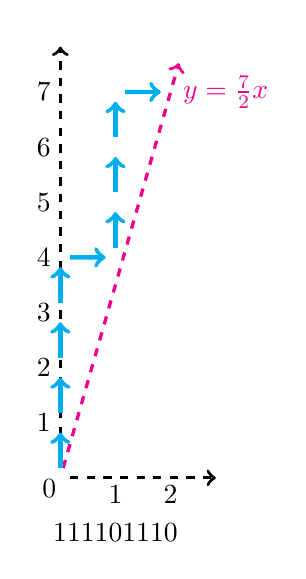
\begin{tikzpicture}[scale = 0.7]
    \node (a) at (0, 0) {};
    \node (b) at (0, 8) {};
    \node (c) at (3, 0) {};
    \node (d) at (2.2, 7.7) {};
    \node (e) at (3, 7) [color = magenta]
        {$y = \frac{7}{2}x$}; 
    \draw [dashed, very thick, ->] (a) to (b);
    \draw [dashed, very thick, ->] (a) to (c);
    \draw [dashed, very thick, ->]
        [color = magenta] (a) to (d);

    \node (1)  at (0,0)   {};
    \node (2)  at (0,1)   {};
    \node (3)  at (0,2)   {};
    \node (4)  at (0,3)   {};
    \node (5)  at (0,4)   {};
    \node (6)  at (1,4)   {};
    \node (7)  at (1,5)   {};
    \node (8)  at (1,6)   {};
    \node (9)  at (1,7)   {};
    \node (10) at (2,7)   {};
    \draw [->, ultra thick, color = cyan]
        (1)  to (2);
    \draw [->, ultra thick, color = cyan] 
        (2)  to (3);
    \draw [->, ultra thick, color = cyan]
        (3)  to (4);
    \draw [->, ultra thick, color = cyan]
        (4)  to (5);
    \draw [->, ultra thick, color = cyan]
        (5)  to (6);
    \draw [->, ultra thick, color = cyan]
        (6)  to (7);
    \draw [->, ultra thick, color = cyan]
        (7)  to (8);
    \draw [->, ultra thick, color = cyan]
        (8)  to (9);
    \draw [->, ultra thick, color = cyan]
        (9)  to (10);

    \node at (-0.2, -0.2) {$0$};
    \node at (-0.3, 1)    {$1$};
    \node at (1, -0.3)    {$1$};
    \node at (-0.3, 2)    {$2$};
    \node at (2, -0.3)    {$2$};
    \node at (-0.3, 3)    {$3$};
    \node at (-0.3, 4)    {$4$};
    \node at (-0.3, 5)    {$5$};
    \node at (-0.3, 6)    {$6$};
    \node at (-0.3, 7)    {$7$};
    \node at (1, -1)      {$111101110$};

\end{tikzpicture}
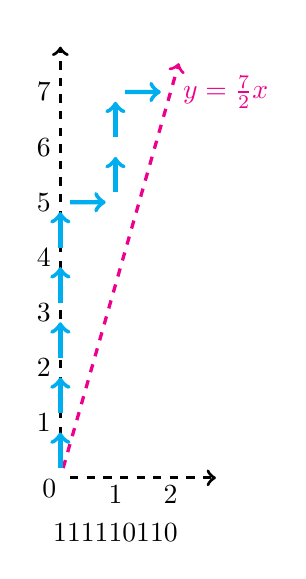
\begin{tikzpicture}[scale = 0.7]
    \node (a) at (0, 0) {};
    \node (b) at (0, 8) {};
    \node (c) at (3, 0) {};
    \node (d) at (2.2, 7.7) {};
    \node (e) at (3, 7) [color = magenta]
        {$y = \frac{7}{2}x$}; 
    \draw [dashed, very thick, ->] (a) to (b);
    \draw [dashed, very thick, ->] (a) to (c);
    \draw [dashed, very thick, ->]
        [color = magenta] (a) to (d);

    \node (1)  at (0,0)   {};
    \node (2)  at (0,1)   {};
    \node (3)  at (0,2)   {};
    \node (4)  at (0,3)   {};
    \node (5)  at (0,4)   {};
    \node (6)  at (0,5)   {};
    \node (7)  at (1,5)   {};
    \node (8)  at (1,6)   {};
    \node (9)  at (1,7)   {};
    \node (10) at (2,7)   {};
    \draw [->, ultra thick, color = cyan]
        (1)  to (2);
    \draw [->, ultra thick, color = cyan] 
        (2)  to (3);
    \draw [->, ultra thick, color = cyan]
        (3)  to (4);
    \draw [->, ultra thick, color = cyan]
        (4)  to (5);
    \draw [->, ultra thick, color = cyan]
        (5)  to (6);
    \draw [->, ultra thick, color = cyan]
        (6)  to (7);
    \draw [->, ultra thick, color = cyan]
        (7)  to (8);
    \draw [->, ultra thick, color = cyan]
        (8)  to (9);
    \draw [->, ultra thick, color = cyan]
        (9)  to (10);

    \node at (-0.2, -0.2) {$0$};
    \node at (-0.3, 1)    {$1$};
    \node at (1, -0.3)    {$1$};
    \node at (-0.3, 2)    {$2$};
    \node at (2, -0.3)    {$2$};
    \node at (-0.3, 3)    {$3$};
    \node at (-0.3, 4)    {$4$};
    \node at (-0.3, 5)    {$5$};
    \node at (-0.3, 6)    {$6$};
    \node at (-0.3, 7)    {$7$};
    \node at (1, -1)      {$111110110$};

\end{tikzpicture}
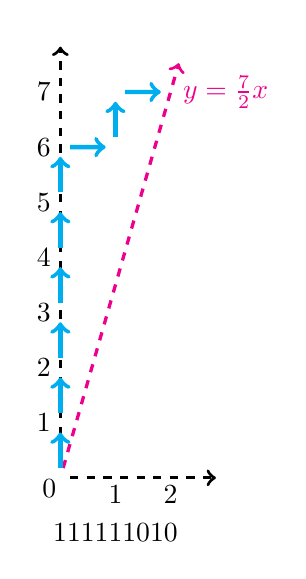
\begin{tikzpicture}[scale = 0.7]
    \node (a) at (0, 0) {};
    \node (b) at (0, 8) {};
    \node (c) at (3, 0) {};
    \node (d) at (2.2, 7.7) {};
    \node (e) at (3, 7) [color = magenta]
        {$y = \frac{7}{2}x$}; 
    \draw [dashed, very thick, ->] (a) to (b);
    \draw [dashed, very thick, ->] (a) to (c);
    \draw [dashed, very thick, ->]
        [color = magenta] (a) to (d);

    \node (1)  at (0,0)   {};
    \node (2)  at (0,1)   {};
    \node (3)  at (0,2)   {};
    \node (4)  at (0,3)   {};
    \node (5)  at (0,4)   {};
    \node (6)  at (0,5)   {};
    \node (7)  at (0,6)   {};
    \node (8)  at (1,6)   {};
    \node (9)  at (1,7)   {};
    \node (10) at (2,7)   {};
    \draw [->, ultra thick, color = cyan]
        (1)  to (2);
    \draw [->, ultra thick, color = cyan] 
        (2)  to (3);
    \draw [->, ultra thick, color = cyan]
        (3)  to (4);
    \draw [->, ultra thick, color = cyan]
        (4)  to (5);
    \draw [->, ultra thick, color = cyan]
        (5)  to (6);
    \draw [->, ultra thick, color = cyan]
        (6)  to (7);
    \draw [->, ultra thick, color = cyan]
        (7)  to (8);
    \draw [->, ultra thick, color = cyan]
        (8)  to (9);
    \draw [->, ultra thick, color = cyan]
        (9)  to (10);

    \node at (-0.2, -0.2) {$0$};
    \node at (-0.3, 1)    {$1$};
    \node at (1, -0.3)    {$1$};
    \node at (-0.3, 2)    {$2$};
    \node at (2, -0.3)    {$2$};
    \node at (-0.3, 3)    {$3$};
    \node at (-0.3, 4)    {$4$};
    \node at (-0.3, 5)    {$5$};
    \node at (-0.3, 6)    {$6$};
    \node at (-0.3, 7)    {$7$};
    \node at (1, -1)      {$111111010$};

\end{tikzpicture}
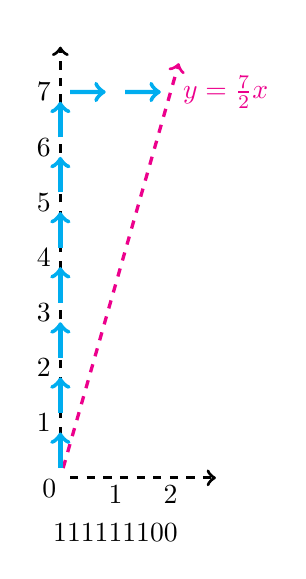
\begin{tikzpicture}[scale = 0.7]
    \node (a) at (0, 0) {};
    \node (b) at (0, 8) {};
    \node (c) at (3, 0) {};
    \node (d) at (2.2, 7.7) {};
    \node (e) at (3, 7) [color = magenta]
        {$y = \frac{7}{2}x$}; 
    \draw [dashed, very thick, ->] (a) to (b);
    \draw [dashed, very thick, ->] (a) to (c);
    \draw [dashed, very thick, ->]
        [color = magenta] (a) to (d);

    \node (1)  at (0,0)   {};
    \node (2)  at (0,1)   {};
    \node (3)  at (0,2)   {};
    \node (4)  at (0,3)   {};
    \node (5)  at (0,4)   {};
    \node (6)  at (0,5)   {};
    \node (7)  at (0,6)   {};
    \node (8)  at (0,7)   {};
    \node (9)  at (1,7)   {};
    \node (10) at (2,7)   {};
    \draw [->, ultra thick, color = cyan]
        (1)  to (2);
    \draw [->, ultra thick, color = cyan] 
        (2)  to (3);
    \draw [->, ultra thick, color = cyan]
        (3)  to (4);
    \draw [->, ultra thick, color = cyan]
        (4)  to (5);
    \draw [->, ultra thick, color = cyan]
        (5)  to (6);
    \draw [->, ultra thick, color = cyan]
        (6)  to (7);
    \draw [->, ultra thick, color = cyan]
        (7)  to (8);
    \draw [->, ultra thick, color = cyan]
        (8)  to (9);
    \draw [->, ultra thick, color = cyan]
        (9)  to (10);

    \node at (-0.2, -0.2) {$0$};
    \node at (-0.3, 1)    {$1$};
    \node at (1, -0.3)    {$1$};
    \node at (-0.3, 2)    {$2$};
    \node at (2, -0.3)    {$2$};
    \node at (-0.3, 3)    {$3$};
    \node at (-0.3, 4)    {$4$};
    \node at (-0.3, 5)    {$5$};
    \node at (-0.3, 6)    {$6$};
    \node at (-0.3, 7)    {$7$};
    \node at (1, -1)      {$111111100$};

\end{tikzpicture}
    \end{center}
\end{example}

\begin{example}[Définition 12 : $a < b : a = 3, b = 5$]
    $w = 20130000$ :\\
    \begin{center}
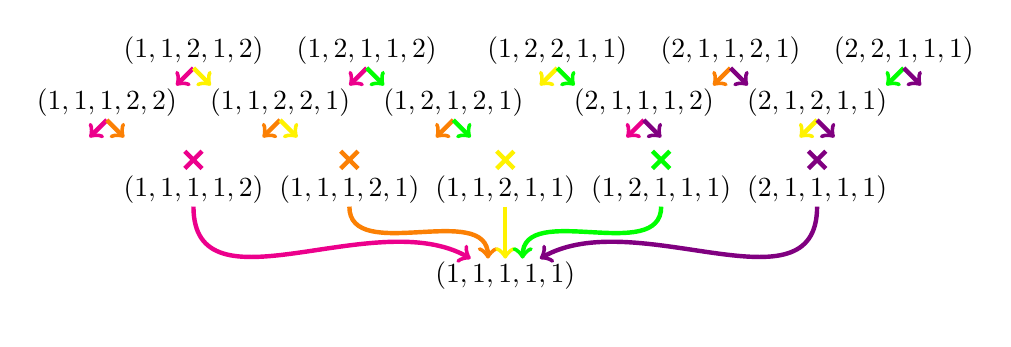
\begin{tikzpicture}[scale = 0.22]
    \node at (0,0) {$(1,1,1,1,1)$};

    \node at (-18,5) {$(1,1,1,1,2)$};
    \node at (-9,5)  {$(1,1,1,2,1)$};
    \node at (0,5)   {$(1,1,2,1,1)$};
    \node at (9,5)   {$(1,2,1,1,1)$};
    \node at (18,5)  {$(2,1,1,1,1)$};

    \node at (-23,10) {$(1,1,1,2,2)$};
    \node at (-18,13) {$(1,1,2,1,2)$};
    \node at (-13,10) {$(1,1,2,2,1)$};
    \node at (-8,13)  {$(1,2,1,1,2)$};
    \node at (-3,10)  {$(1,2,1,2,1)$};
    \node at (3,13)   {$(1,2,2,1,1)$};
    \node at (8,10)   {$(2,1,1,1,2)$};
    \node at (13,13)  {$(2,1,1,2,1)$};
    \node at (18,10)  {$(2,1,2,1,1)$};
    \node at (23,13)  {$(2,2,1,1,1)$};

    \draw [->][color=magenta, ultra thick]
        (-23,9) to (-24,8);
    \draw [->][color=magenta, ultra thick]
        (-18,12) to (-19,11);
    \draw [->][color=magenta, ultra thick]
        (-8,12) to (-9,11);
    \draw [->][color=magenta, ultra thick]
        (8,9) to (7,8);
    \draw[color=magenta, ultra thick]
        (-18.5,7.2) -- (-17.5,6.2);
    \draw[color=magenta, ultra thick]
        (-18.5,6.2) -- (-17.5,7.2);
    \draw [->][out=-90,in=150, ultra thick] 
        [color=magenta](-18,4) to (-2,1);

    \draw [->][color=brown!7!orange, ultra thick]
        (-23,9) to (-22,8);
    \draw [->][color=brown!7!orange, ultra thick]
        (-13,9) to (-14,8);
    \draw [->][color=brown!7!orange, ultra thick]
        (-3,9) to (-4,8);
    \draw [->][color=brown!7!orange, ultra thick]
        (13,12) to (12,11);
    \draw[color=brown!7!orange, ultra thick]
        (-9.5,7.2) -- (-8.5,6.2);
    \draw[color=brown!7!orange, ultra thick]
        (-9.5,6.2) -- (-8.5,7.2);
    \draw [->][out=-90,in=90, ultra thick]
        [color=brown!7!orange](-9,4) to (-1,1);

    \draw [->][color=yellow, ultra thick]
        (-18,12) to (-17,11); 
    \draw [->][color=yellow, ultra thick]
        (-13,9) to (-12,8); 
    \draw [->][color=yellow, ultra thick]
        (3,12) to (2,11); 
    \draw [->][color=yellow, ultra thick]
        (18,9) to (17,8); 
    \draw[color=yellow, ultra thick]
        (-0.5,7.2) -- (0.5,6.2);
    \draw[color=yellow, ultra thick]
        (-0.5,6.2) -- (0.5,7.2);
    \draw [->][out=-90,in=90, ultra thick] 
        [color=yellow](0,4) to (0,1);

    \draw [->][color = green,  ultra thick]
        (-8,12) to (-7,11);
    \draw [->][color=green, ultra thick]
        (-3,9) to (-2,8);
    \draw [->][color=green, ultra thick]
        (3,12) to (4,11);
    \draw [->][color=green, ultra thick]
        (23,12) to (22,11);
    \draw[color=green, ultra thick]
        (8.5,7.2) -- (9.5,6.2);
    \draw[color=green, ultra thick]
        (8.5,6.2) -- (9.5,7.2);
    \draw [->][out=-90,in=90, ultra thick]
        [color=green](9,4) to (1,1);

    \draw [->][color=violet, ultra thick]
        (8,9) to (9,8);
    \draw [->][color=violet, ultra thick]
        (13,12) to (14,11);
    \draw [->][color=violet, ultra thick]
        (18,9) to (19,8);
    \draw [->][color=violet, ultra thick]
        (23,12) to (24,11);
    \draw[color=violet, ultra thick]
        (17.5,7.2) -- (18.5,6.2);
    \draw[color=violet, ultra thick]
        (17.5,6.2) -- (18.5,7.2);
    \draw [->][out=-90,in=30, ultra thick] 
        [color=violet](18,4) to (2,1);

\end{tikzpicture}
\end{center}
   \end{example}

\begin{example}[Définition 12 : $a > b : a = 7, b = 3$]
    $w_2 = 2456017030$ :\\
 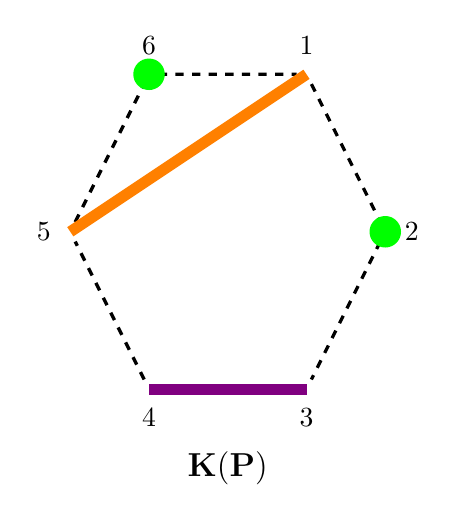
\begin{tikzpicture}[scale=1]
    \node at (3,0) {\large $\mathbf{K(P)}$};
    \node [label = above : {$1$}] (1)
        at (4,5) {};
    \node [label = right : {$2$}] (2)
        at (5,3) {};
    \node [label = below : {$3$}] (3)
        at (4,1) {};
    \node [label = below : {$4$}] (4)
        at (2,1) {};
    \node [label = left : {$5$}]  (5)
        at (1,3) {};
    \node [label = above : {$6$}] (6)
        at (2,5) {};
    \draw [dashed][very thick]
    (1) -- (2) -- (3) -- (4)
        -- (5) -- (6) -- (1);
    \draw [color = orange][line width = 4pt] 
        (4,5) -- (1,3);            
    \draw [color = violet][line width = 4pt] 
        (4,1) -- (2,1);
    \fill [color=green] (5,3) circle (0.2); 
    \fill [color=green] (2,5) circle (0.2);   
  \end{tikzpicture}
\end{example}

\begin{example}[Théorème 9 : $a = 4, b = 3$]
    $lr_{a,b} = 3^3 = 27$
    \begin{itemize}
        \item Mots de la forme $XXXX000$ :
            \subitem $1234000$
        \item Mots de la forme $XXX0X00$ :
            \subitem $1230400$
            \hspace{2cm} $1240300$
            \hspace{2cm} $1340200$
            \subitem $2340100$
        \item Mots de la forme $XX0XX00$ :
            \subitem $1203400$
            \hspace{2cm} $1302400$
            \hspace{2cm} $1402300$
            \subitem $2301400$
            \hspace{2cm} $2401300$
            \hspace{2cm} $3401200$
        \item Mots de la forme $XXX00X0$ :
            \subitem $1230040$
            \hspace{2cm} $1240030$
            \hspace{2cm} $1340020$
            \subitem $2340010$
        \item Mots de la forme $XX0X0X0$ :
            \subitem $1203040$
            \hspace{2cm} $1204030$
            \hspace{2cm} $1302040$
            \subitem $1304020$
            \hspace{2cm} $1402030$
            \hspace{2cm} $1403020$
            \subitem $2301040$
            \hspace{2cm} $2304010$
            \hspace{2cm} $2401030$
            \subitem $2403010$
            \hspace{2cm} $3401020$
            \hspace{2cm} $3402010$
    \end{itemize}
    
\end{example}